\hebrewsection{Wireless Communication and Fading Channels}

The wireless channel is far more challenging than the stationary AWGN channel due to mobility and multipath propagation.

\subsection{Multipath Propagation and Fading}
In a wireless environment, the signal reaches the receiver via multiple paths (reflection, diffraction, scattering). These paths have different delays, phases, and amplitudes.

\subsubsection{Rayleigh Fading}
When there is no line-of-sight (LOS) component, the received signal envelope follows a Rayleigh distribution. This is typical in dense urban environments.

\subsubsection{Ricean Fading}
When a dominant LOS path exists, the envelope follows a Ricean distribution, characterized by the $K$-factor (ratio of LOS power to multipath power).

\subsection{Small-Scale Fading Parameters}
\begin{itemize}
    \item \textbf{Delay Spread:} The difference in arrival times of the paths. It leads to \textbf{frequency-selective fading} if the bandwidth exceeds the coherence bandwidth.
    \item \textbf{Doppler Spread:} Caused by mobility, leading to frequency shifts. It causes \textbf{time-selective fading} if the symbol duration exceeds the coherence time.
\end{itemize}

\subsection{Diversity Techniques}
Diversity is the primary tool to combat fading by providing multiple independent copies of the signal.
\begin{enumerate}
    \item \textbf{Temporal Diversity:} Interleaving and coding.
    \item \textbf{Frequency Diversity:} OFDM and spread spectrum.
    \item \textbf{Spatial (Antenna) Diversity:} Using multiple antennas (MIMO).
\end{enumerate}

\subsubsection{MIMO: Multiple-Input Multiple-Output}
MIMO systems use multiple antennas at the transmitter and receiver.
\begin{itemize}
    \item \textbf{Spatial Multiplexing:} Increases data rate by sending independent streams.
    \item \textbf{Beamforming:} Focuses energy in a specific direction to increase SNR.
    \item \textbf{Space-Time Coding:} Increases reliability (e.g., Alamouti scheme).
\end{itemize}

\begin{center}
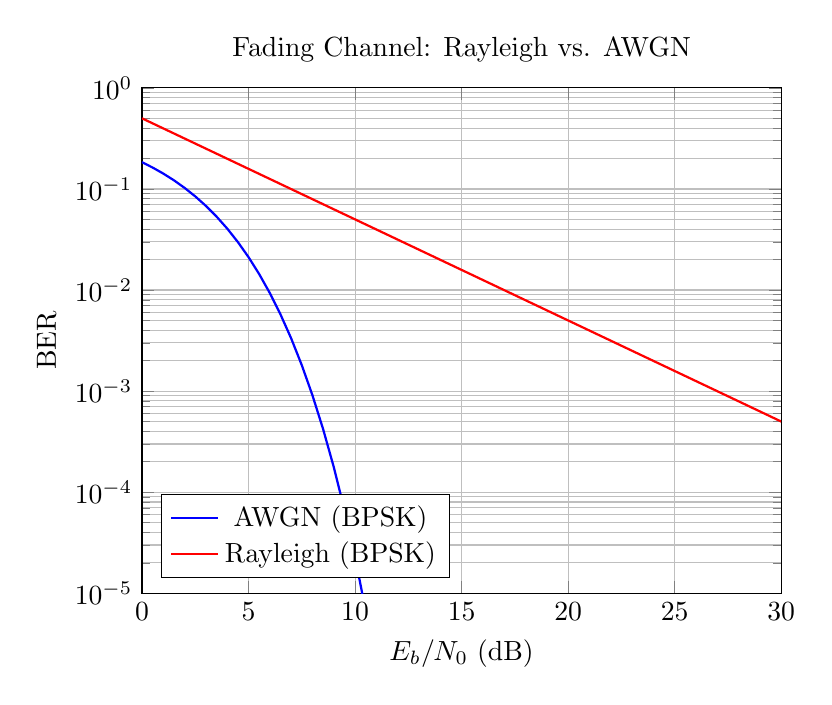
\begin{tikzpicture}
\begin{axis}[
    title={Fading Channel: Rayleigh vs. AWGN},
    xlabel={$E_b/N_0$ (dB)},
    ylabel={BER},
    ymode=log,
    grid=both,
    xmin=0, xmax=30,
    ymin=1e-5, ymax=1,
    width=0.8\textwidth,
    height=8cm,
    legend pos=south west
]
\addplot[blue, thick, domain=0:12] {0.5 * exp(-10^(x/10))};
\addlegendentry{AWGN (BPSK)}
\addplot[red, thick, samples=100, domain=0:30] {0.5 / (10^(x/10))};
\addlegendentry{Rayleigh (BPSK)}
\end{axis}
\end{tikzpicture}
\end{center}

\subsection{Channel Estimation and Equalization}
In fading channels, the receiver must estimate the channel's complex gain (CSI - Channel State Information) to perform coherent demodulation. Pilots (known symbols) are periodically transmitted for this purpose. Adaptive equalizers then invert the channel's impact.
